\documentclass{report}

\usepackage{url}
\usepackage{indentfirst}
\usepackage{float}

\usepackage[T1]{fontenc}
\usepackage{textcomp} % Required for upquote.
\usepackage{listings} % Include the listings-package
% Ensure quotes in listings are straight.
% Cleaner way to print strings in listings packages so no space symbol.
\lstset{showstringspaces=false, 
        upquote=true} 


\usepackage{mdframed}
\usepackage[numbers,sort]{natbib}
%\usepackage[english]{babel} % Need for text wrap in table.
\usepackage{array} % Needed for centering in the table
\usepackage[export]{adjustbox} % loads also graphicx
\usepackage{graphicx}

\usepackage{hyperref} % Creates links in the PDF document.
\hypersetup{hidelinks} % Do not include boxes around links

% Defines the table of contents depth and the subsection numbering depth
\setcounter{secnumdepth}{5}
\setcounter{tocdepth}{5}

\title{\emph{HamSkill}: Run Haskell Anywhere \\
with ANTLR and Scala\\[1in]
	   CS252 Project Final Report}

\author{
  Zayd Hammoudeh \\
  (zayd.hammoudeh@sjsu.edu)
  }


\newcommand{\myparagraph}[1]{\paragraph{#1}\mbox{}\\}

% Skip lines after each paragraph.
\setlength\parskip{\baselineskip}

\begin{document}

\maketitle

\pagenumbering{roman}

\tableofcontents{\protect\newpage}

\addcontentsline{toc}{section}{List of Figures}
\listoffigures
\newpage
 
\pagenumbering{arabic}

\renewcommand\thesection{\arabic{section}}

\section{Running in the Java Virtual Machine}\label{sec:jvm}

C is one of the most commonly used languages when the primary objective is maximum performance.  However, C's ``write once, compile anywhere'' paradigm limits its portability.  In contrast, the near ubiquity of the Java Virtual Machine (JVM) allows Java to be ``write once, run anywhere.''  

Developers have often leveraged the JVM's ``run anywhere'' capability for other languages than Java.  Examples include: JRuby for the Ruby programming language \cite{jruby}, Jython for the Python programming language \cite{jython_jvm}, Renjin for the R programming language \cite{renjin}, and Scala \cite{scala}.

Currently, there is no full implementation of Haskell in the JVM.  One Haskell dialect that is runnable in Java is Frege \cite{frege}.  

This project implements, \emph{HamSkill}, which is a transpiler from Haskell to Scala; \textit{HamSkill} enables a dialect of Haskell to run in the JVM.  

\section{Key Project Requirements}\label{sec:keyProjectRequirements}

When designing and implementing this project, there were four primary goals:

\begin{enumerate}

\item \textbf{Runnable in the Java Virtual Machine} - As explained in Section~\ref{sec:jvm}, Java's Virtual Machine enables significant machine independence, which Haskell does not currently have.

\item \textbf{Minimal JVM Requirements} - In addition to just running in the JVM, \textit{HamSkill} was created to be as standalone as possible.  As an example, it was not expected that in most applications, the user would have Scala installed on their machine.  To achieve this maximum portability, some more niche features of Haskell may not be supported.

\item \textbf{Identical Input and Output Between Haskell and \emph{HamSkill}} - In many scenarios, it may not be sufficient for a Haskell program to simply run inside the JVM.  Rather, it is more likely that the output generated by the two environments will need to be identical.  As such, \emph{HamSkill} includes an additional post-processing step to ensure its output is identical to that of Haskell.

\item \textbf{Human Readable Output Code} - A transpiler is any program that takes source code from one programming language and outputs code in another programming language, with a similar level of abstraction \cite{jansen_2015}.  To enable increased reuse of the outputted code, \textit{HamSkill} uses techniques such as indenting, newlines, etc. to maximize the readability of the generated output.  While this is not a necessary requirement for the complete system to work properly, it enhances the tool's potential.

\end{enumerate}

\section{\textit{HamSkill}'s Software Architecture}\label{sec:hamskillSoftwareArchitecture}

\emph{HamSkill} is a transpiler that takes Haskell code as an input, converts it to Scala, and then runs the transpiled code in the JVM.  The \emph{HamSkill} implementation consists of six major components.  They are:

\begin{itemize}
   \item ANTLR Lexer and Parser
   \item \texttt{Haskell} ANTLR Grammar
   \item \texttt{ScalaOutput} ANTLR Grammar
   \item Scala Runtime Environment
   \item \texttt{HamskillMain} Java Class
   \item \texttt{ScalaOutput} Java Class
\end{itemize}

The relationships between these components are shown in Figure~\ref{fig:hamskillArchitecture}, and the following subsections describe the role of each component in the overall system.

\begin{figure}[ht!]
	\centering
		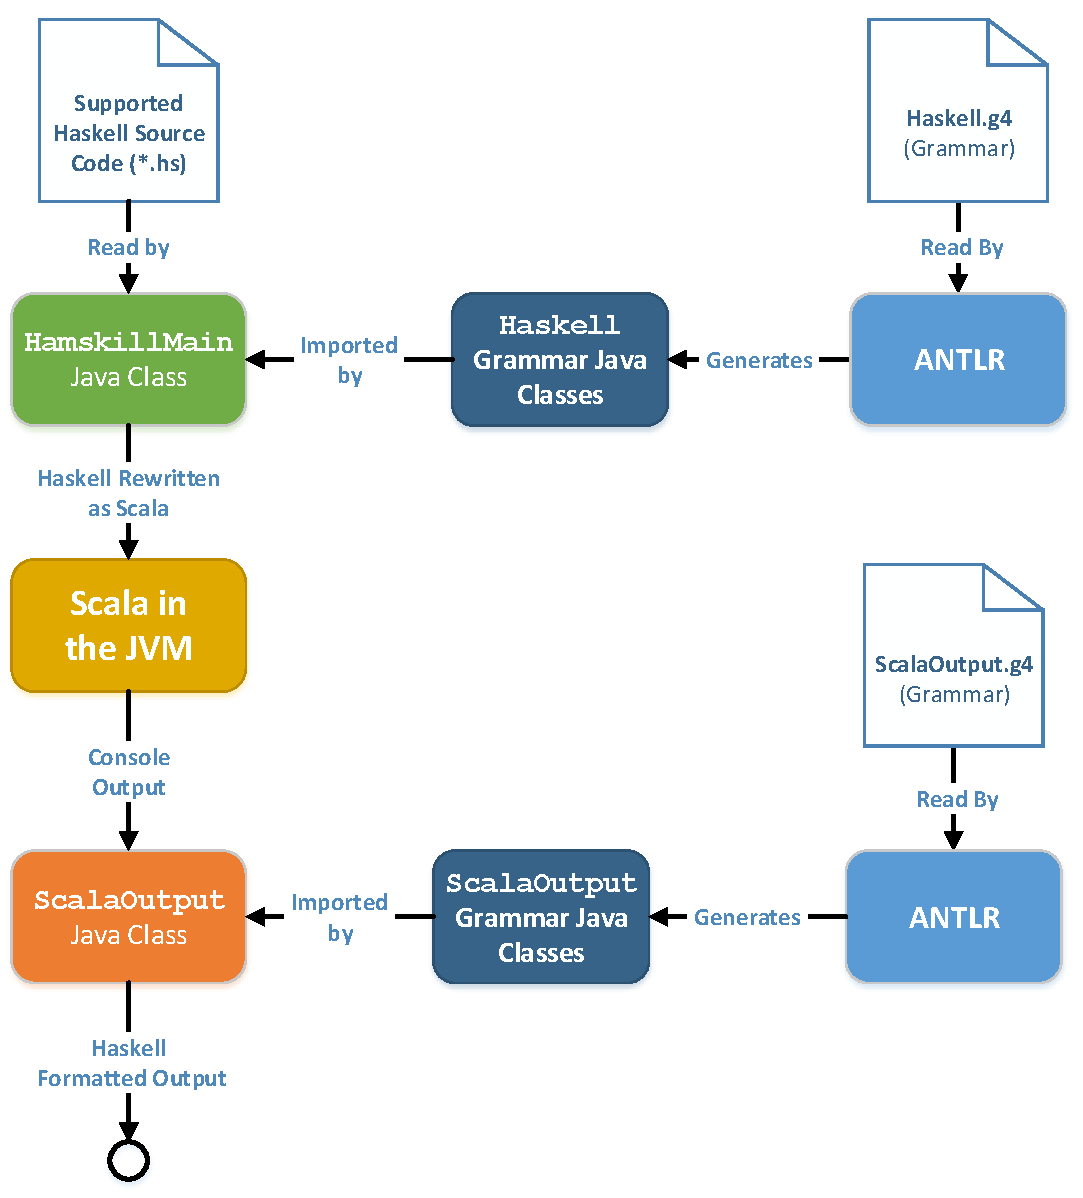
\includegraphics[width=1.0\textwidth]{images/cs252_project_diagram_cropped.pdf}
	\caption{\textit{HamSkill} Project Architecture}\label{fig:hamskillArchitecture}
\end{figure}

\subsection{ANTLR}

ANTLR (\underline{AN}other \underline{T}ool for \underline{L}anguage \underline{R}ecognition) is an adaptive left-to-right, left-most deriviation (LL(*)) lexer and parser written in the Java programming language.  ANTLR's primary function is to read, parse, and process structured text (e.g. Haskell code) \cite{antlrDefinitiveReference}.  

\subsubsection{ANTLR Version 4 Grammar}

A grammar is a formal description of sentences in a language; it is based off the concept of a context-free grammar in automata theory.  ANTLR version 4's (v4) grammar files (denoted by the file extension ``\emph{.g4}'') explicitly define how ANTLR will parse some structured text.  The grammar file may contain token definitions (which always start with a capital letter) and/or parser rules (which always start with a lowercase letter).  A token is a group of characters that form a single object; the parser uses these tokens to recognize sentence structures within a corpus.

This project utilizes two separate grammars namely: \texttt{Haskell} and \texttt{ScalaOutput}.  These grammars are described in the following two subsections.

\myparagraph{\textit{HamSkill}'s \texttt{Haskell} Grammar}\label{sec:haskellG4}

The custom ANTLR grammar, \texttt{Haskell}, was created for this project and is contained in the file ``\texttt{Haskell.g4}.''  This grammar defines both the tokens and abstract syntax tree for supported Haskell code.  Some of the Haskell language features that this grammar supports include:

\begin{itemize}
   \item \texttt{case} Statements
   \item \texttt{if}, \texttt{then}, \texttt{else} Conditionals
   \item \texttt{Maybe} Monads
   \item Currying
   \item Partially Applied Functions
   \item Higher Order Functions
   \item Lazy Evaluation
\end{itemize}

For the complete feature set as well as any Haskell syntax requirements, see Section~\ref{sec:hamskillFeatures}.

\myparagraph{\textit{HamSkill}'s \texttt{ScalaOutput} Grammar} 

As mentioned in Section~\ref{sec:keyProjectRequirements}, one of the key requirements of this project was that the outputs from Haskell and \textit{HamSkill} be identical.  Figures~\ref{fig:printListHaskell} and~\ref{fig:printListScala} show the Haskell and Scala code respectively to print a list containing integers ``2'', ``3'', and ``4'' to the console.  Note that the second line in the two figures (which shows each language's respective console output) are very different.

\begin{figure}[H]
\begin{mdframed}
\begin{lstlisting}[language=Haskell]
Prelude> putStrLn $ show [2, 3, 4]
[2,3,4]
\end{lstlisting}
\end{mdframed}
\caption{Printing a Three Element List in Haskell}\label{fig:printListHaskell}
\end{figure}

\begin{figure}[H]
\begin{mdframed}
\begin{lstlisting}[language=Scala]
scala> println(List(2,3,4))
List(2, 3, 4)
\end{lstlisting}
\end{mdframed}
\caption{Printing a Three Element List in Scala}\label{fig:printListScala}
\end{figure}

The ANTLR grammar, \texttt{ScalaOutput}, (contained in the file ``\texttt{ScalaOutput.g4}'') is used to account for these types of differences by parsing the console output of a Scala program and converting that output to a syntax that is more similar to that of Haskell.

\subsubsection{ANTLR-Generated Java Classes}

Programs that use ANTLR do not generally operate directly on the grammar.  Rather, the grammar is converted by ANTLR into a set of Java classes; given an  grammar (e.g. ``\emph{GrammarName.g4}''),  ANTLR creates the following files:

\begin{itemize}
	\item \emph{GrammarName}Lexer.java - This class is the lexer defined by the input grammar file.  It extends ANTLR's base \texttt{Lexer} class.
	
	\item \emph{GrammarName}Parser.java - Each rule in the original grammar constitutes a method in this class; it forms the parser class definition associated with the input grammar file.
	
	\item \emph{GrammarName}.tokens - Assigns a token type (e.g. integer, identifier, floating point number, etc.) to each token in the input grammar file.
	
	\item \emph{GrammarName}Listener.java \& \emph{GrammarName}BaseListener.java - ANTLR applies the grammar to a text input to build an Abstract Syntax Tree (AST).  While walking the tree, ANTLR fires events that are captured by a listener in these two classes \cite{antlrDefinitiveReference}.
	
\end{itemize}

Most programs that use ANTLR override at least some of the functions in the file ``\emph{GrammarName}BaseListener.java.''


\myparagraph{\texttt{HaskellTokensToScala} Java Class}

The class ``\texttt{HaskellTokensToScala}'' overrides some of the methods that ANTLR auto-generated in the file ``\texttt{HaskellBaseListener.java}''; note that all of these overridden methods are derived from the grammar ``\texttt{Haskell.g4}'' described in Section~\ref{sec:haskellG4}.  In the end, it is the Java code in this file that performs the actual, low-level transpilation from Haskell to Scala.

\eject
\myparagraph{\texttt{ScalaOutputTokensToHaskellFormat} Java Class}\label{sec:scalaOutputFunctionality}

Similar to the \texttt{HaskellTokensToScala} class, the class, ``\texttt{ScalaOutputTokensToHaskellFormat}'' extends the ANTLR auto-generated class, ``\texttt{ScalaOutputBaseListener}''.

The listeners in the \texttt{ScalaOutputTokensToHaskellFormat} class are primarily responsible for transforming two different categories of Scala console outputs, specifically:

\begin{itemize}

\item \textbf{Lists} - As shown in Figures~\ref{fig:printListHaskell} and~\ref{fig:printListScala}, the console output of lists in Scala and Haskell are significantly different.  The methods in this class, coupled with the \texttt{ScalaOutput} grammar, convert printed lists from Scala to Haskell format.

\item \textbf{\texttt{Maybe}} Monad - Scala's approximate equivalent of Haskell's \texttt{Maybe} monad is named \texttt{Option}.  While the syntax for the two are similar, they are not identical.  For example, ``\texttt{Just}'' and ``\texttt{Nothing}'' in Haskell are referred to as ``\texttt{Some}'' and ``\texttt{None}'' in Scala.  The monad naming convention conversion for console outputs from Scala back to Haskell is handled by the \texttt{ScalaOutput} class.

\end{itemize}

Any other Scala console outputs that do not fall into these two categories are passed through unchanged.


\subsection{Transpiler Output Language: Scala}

As defined previously, a transpiler takes source code from one programming language and converts it to code in another language.  It was also previous explained that the primary criteria when deciding on \textit{HamSkill}'s output language was that it needed to be runnable in the Java Virtual Machine.  Other important criteria that guided language selection were:

\begin{itemize}

	\item \textbf{Higher-Order Function Support} - Any language that is devoid of higher-order function support would be a poor match for a purely functional language like Haskell.
	
	\item \textbf{Similar Syntactic Structure} - Closer alignment between the input and output languages simplifies the transpilation.  Inevitably though, some degree of restructuring and reformatting is required.  
	
	\item \textbf{Personal Interest} - Increased student interest in a project topic generally leads to a more fulfilling outcome for the student and also a better project overall.  

\end{itemize}

The language that best fit these criteria is Scala, which is a functional language that is run inside the JVM \cite{whatIsScala}. What is more, Scala natively supports many of Haskell's core features including: functions written in a pattern matching style, immutability of objects, currying, partially applied functions, lazy evaluation, static typing, etc.  One of the disadvantages of Scala is its weaker type inference in comparison to Haskell; due to this, specific requirements were placed on the Haskell dialect supported by \textit{HamSkill} as described in Section~\ref{sec:hamskillFeatures}.  It must be noted that the author has a predisposed interest towards learning Scala given its extensive support by Apache Spark.  Given all of these factors, the selection of Scala for this project became an obvious choice.\footnote{Special recognition to Dr. Thomas Austin is required for pointing the author in the direction of Scala.}

\textit{HamSkill} implements two different schemes for running the transpiled Scala code, namely \textit{HamSkill} Standard and \textit{HamSkill}+.  They are described in the following subsections.

\subsubsection{\textit{HamSkill} Standard}

Since Scala is a compiled language, it is limited in its ability to perform runtime compilation and execution via Java.  To overcome this challenge, \textit{HamSkill} leverages Twitter's \texttt{util-eval} library, which allows runtime compilation and execution of Scala code entirely within a Java program \cite{githubTwitterEvalUtil}.  This approach is known as ``\textit{HamSkill} Standard''; the advantages and disadvantages of using the \texttt{util-eval} library include:

\begin{itemize}

\item \textbf{Advantages}:

\begin{enumerate}

\item \textbf{Reduced JVM Requirements} - Twitter's \texttt{util-eval} library is a JAR file that only requires the presence of Scala's compile and main library JAR files to run.  Hence, this eliminates the need for the user to have Scala installed in their environment.  This addresses one of the key requirements enumerated in Section~\ref{sec:keyProjectRequirements}.

\item \textbf{Simplified Usage} - When running \textit{HamSkill} Standard, only a single function call is required to transpile, compile, then run the Scala code.  In contrast, \textit{HamSkill}+ needs at least four steps to do the same task, which inevitably introduces additional possible points of error.

\end{enumerate}

\item \textbf{Disadvantages}:

\begin{enumerate}

\item \textbf{Reduced Feature Set} - The \texttt{util-eval} library does not support all Scala features.  An example of a missing feature is the function ``\texttt{readLine}'', which takes console inputs.

\item \textbf{Reliance on Third Party Developers} - As mentioned previously, \texttt{util-eval} was developed by Twitter.  Hence, it can be deprecated at any time (as Twitter had previously planned \cite{deprecateUtilEval}).  While the library is open-source, picking up a dropped project introduces an additional set of complications.

\end{enumerate}

\end{itemize}

\subsubsection{\textit{HamSkill}+}

Unlike \textit{HamSkill} Standard, \textit{HamSkill}+ requires Scala to be installed on the host PC.  What this enables is that any feature that is supported by the installed version of Scala could in theory be utilized by \textit{HamSkill}+.  Currently, running a Haskell program with \textit{HamSkill}+ requires four separate steps, all of which are controlled by a \texttt{bash} script as shown in Figures~\ref{fig:runHamSkill},~\ref{fig:compileScala}, and~\ref{fig:runScalaAndConvertOutput}; these steps are:

\begin{enumerate}

\item \textbf{Transpile the Haskell code to Scala} - This is done by running the \texttt{main} method in the \texttt{HamskillMain} class as shown in Figure~\ref{fig:runHamSkill}.  Note that ``\texttt{"\$@"}'' is \texttt{bash} notation that entails that any parameters passed to the \texttt{bash} script are directly passed as arguments into the JAR's \texttt{main} method.  In \textit{HamSkill}+, the last argument passed to the \texttt{main} method is the name of the file where the transpiled Scala code will be written.

\begin{figure}[H]
\begin{mdframed}
\begin{lstlisting}[language=bash, upquote=true]
java -jar hamskill.jar "$@"
\end{lstlisting}
\end{mdframed}
\caption{Transpiling from Haskell to Scala with \textit{HamSkill}+}\label{fig:runHamSkill}
\end{figure}

\item \textbf{Compile the Transpiled Scala Code} - The \texttt{bash} command to compile Scala is ``\texttt{scalac}'' as shown in Figure~\ref{fig:compileScala}.  Note that ``\texttt{\$scalaSrcFile}'' is the filename where the transpiled Scala code was written in the previous step.

\begin{figure}[H]
\begin{mdframed}
\begin{lstlisting}[language=bash]
scalac $scalaSrcFile
\end{lstlisting}
\end{mdframed}
\caption{Compiling the Transpiled Scala Code in \textit{HamSkill}+}\label{fig:compileScala}
\end{figure}

\item \textbf{Execute the Transpiled Scala Code} - The \texttt{bash} command to run compiled Scala code is simply ``\texttt{scala}'' as shown in Figure~\ref{fig:runScalaAndConvertOutput}.  Note that ``\texttt{\$scalaObject}'' is the name of the encapsulated Scala object (similar to a class in Java) in the compiled Scala file.

\begin{figure}[H]
\begin{mdframed}
\begin{lstlisting}[language=bash]
scala -cp . $scalaObject 
          | java -cp hamskill.jar hamskill.ScalaOutput
\end{lstlisting}
\end{mdframed}
\caption{Executing the Scala Code and Piping the Output to \textit{HamSkill} Java Class ``\texttt{ScalaOutput}''}\label{fig:runScalaAndConvertOutput}
\end{figure}

\item \textbf{Pipe the Scala Output to the \texttt{ScalaOutput} Class} - The console output of the Scala code is piped (via ``\texttt{|}'') into the Java class \texttt{ScalaOutput} as shown in Figure~\ref{fig:runScalaAndConvertOutput}.  As explained in Section~\ref{sec:scalaOutputFunctionality}, this class performs any necessary transformations on the console output(s) and then prints the transformed output to the console as if the original code had been run in Haskell.

\end{enumerate} 


\section{Overview of \textit{HamSkill}'s Test Strategy and Architecture}

Software testing detects defects in software programs; there are different types of software testing including: unit testing, module level testing, and system testing.  Given that ANTLR relies heavily on the Listener pattern, it reduces the ease at which unit testing can be performed.  What is more, given that \textit{HamSkill} relies on the end to end operation of programs written in Haskell, ANTLR, Java, and Scala, it lends itself to a system-level testing methodology.

\subsection{System Level and Regression Testing}

\textit{HamSkill}'s uses black-box system level testing.  A set of use cases (i.e. Haskell files) were generated by the author; these files are then run through both Haskell (to verify they are valid Haskell code) and through \textit{HamSkill}; the resulting outputs are then compared.  If the outputs are the same, the test is considered successful; in the case of any differences, the test is classified as a failure.  The full set of \textit{HamSkill} test cases are included with this submission in the folder \path{Test_Bench/test_cases}.

Regression testing verifies that new features do not affect/compromise existing ones.  When developing \textit{HamSkill}, new features were iteratively added.  After each feature was added, the entire test bench was run to ensure that no new (detectable) issues were introduced.  If an issue did arise, it would be immediately addressed before adding new features to ensure that fundamental problems did not compound upon themselves. This formed a type of regression testing throughout \textit{HamSkill}'s development.

\subsection{Test Bench Implementation Overview}

The \textit{HamSkill} test architecture is written as a \texttt{bash} script (see the file ``\path{Test_Bench/test_bench.sh}'' included with the submission).  The function ``\path{perform_hamskillStd_and_hamskillPlus_test}'' is the most important in the script as it performs most of the testing; the basic operational flow of this function is:

\begin{itemize}

\item \textbf{Step \#1}: Provide the \texttt{bash} function with the name of a Haskell program written in the dialect supported by \textit{HamSkill}, but without the file extension.

\item \textbf{Step \#2}: Run the specified Haskell program through Haskell and store the program's output to a specific file on disk using the \texttt{bash} command ``\texttt{>}''. 

\item\label{item:runHamSkillStandard} \textbf{Step \#3}: Run \textit{HamSkill} Standard and output the results to a different file using the \texttt{bash} command ``\texttt{>}''. 

\item\label{item:diffHamSkillStandard} \textbf{Step \#4}: Perform a file difference operation (using the \texttt{bash} ``\texttt{diff}'' command) on the output files from Haskell and \textit{HamSkill} Standard.  If the two files are identical, then mark the test as passing; if they are different, the test failed.
 
\item \textbf{Step \#5}: Repeat steps \#3 and \#4 using \textit{HamSkill}+.

\end{itemize}

There is an additional function in the \texttt{bash} test bench named ``\texttt{print\_final\_results}'' that prints the number of passing tests versus the total number of tests.

\subsection{Test Cases}

From the perspective of the test bench, a single Haskell file being run through either \textit{HamSkill} Standard or \textit{HamSkill}+ represents a single test case.  In Section~\ref{sec:hamskillFeatures}, the test bench file used to verify each \textit{HamSkill} feature is documented for reference.

\section{Haskell Features Supported by \textit{HamSkill}}\label{sec:hamskillFeatures}

This section enumerates the Haskell features that are supported by \textit{HamSkill}.  It also details any specific formatting requirements for the \textit{HamSkill} Haskell dialect.

\subsection{Single Haskell File}

Currently, \textit{HamSkill} only supports a single Haskell file at a time.  If the user wants to run code across multiple files, s/he could transpile the code to Scala via \textit{HamSkill}, manually configure the imports, and then run the Scala code manually.  While this requirement may be a bit onerous, it should not limit the tool's total capabilities in a meaningful way.

\subsection{Support for Functions}

Functions written in Haskell can be interpreted by \textit{HamSkill}.  Figure~\ref{fig:myFunctionHaskell} is a function from the \textit{HamSkill} test case ``\texttt{simple\_function\_call.hs}''.

\begin{figure}[H]
\begin{mdframed}
\begin{lstlisting}[language=Haskell]
myFunc :: [Int] -> Int -> Int
myFunc x y = 3 + 5
\end{lstlisting}
\end{mdframed}
\caption{Simple Haskell Function Supported by \textit{HamSkill}}\label{fig:myFunctionHaskell}
\end{figure}

The following subsections enumerate the requirements a Haskell function must satisfy to be supported by \textit{HamSkill}.

\subsubsection{Explicit Function Type Signature}\label{sec:explicitTypeSignature}

All functions (excluding partially applied functions as described in Section~\ref{sec:partiallyAppliedFunctions}) must have an explicit type signature.  Note that only a subset of Haskell's base classes are supported (see Section~\ref{sec:supportedTypes} for details on the supported types).  

Currently, type variables (even if they map to a supported type) are not supported.

\subsubsection{Pattern Matching}\label{sec:supportedPatternMatching}

As shown in Figure~\ref{fig:myFunctionHaskell}, pattern matching of function variables is supported.  Special pattern matching cases that \textit{HamSkill} handles include:

\begin{itemize}

\item Ignored variables via the Underscore (\texttt{\_}) Notation

\item Prepend using Colon (\texttt{:})

\item Empty Lists (\texttt{[ ]})

\end{itemize}

Figure~\ref{fig:functionZaydFoldr} is a function from the \textit{HamSkill} test case ``\texttt{partially\_applied\_example.hs}'' that uses all three of the previously mentioned special pattern matching cases.

\begin{figure}[H]
\begin{mdframed}
\begin{lstlisting}[basicstyle=\small, language=Haskell]
zayd_foldr :: (Int -> Int -> Int) -> Int -> [Int] -> Int
zayd_foldr _ acc [] = acc
zayd_foldr f acc (x:xs) = f (x) (zayd_foldr (f) (acc) (xs))
\end{lstlisting}
\end{mdframed}
\caption{\textit{HamSkill} Pattern Matching Example}\label{fig:functionZaydFoldr}
\end{figure}

Guards in Haskell are not currently supported.


\subsubsection{Recursion}

Recursion is supported by \textit{HamSkill}; however, there are requirements on how function parameters must be specified (see Section~\ref{sec:callingAFunction}).

Figures~\ref{fig:functionZaydFoldr} and~\ref{fig:functionAddList} are recursive functions supported by \textit{HamSkill}; note that the function in Figure~\ref{fig:functionAddList} is in the \textit{HamSkill} test case ``\texttt{addList.hs}''.

\begin{figure}[H]
\begin{mdframed}
\begin{lstlisting}[language=Haskell]
addList :: [Int] -> Int
addList [] = 0
addList (x:xs) = x + (((addList xs)))
\end{lstlisting}
\end{mdframed}
\caption{A Recursive Call to a Haskell Function that Sums All Integers in a List}\label{fig:functionAddList}
\end{figure}

\subsubsection{A Single Executable Expression per Pattern Matching Statement}

For each pattern matching case, only a single expression is allowed; Haskell's \texttt{where} and \texttt{let} syntaxes are not supported.  As an example, the first pattern matching case in Figure~\ref{fig:functionZaydFoldr} simply returns ``\texttt{acc}'' while the second pattern matching case returns the result of calling the function ``\texttt{f}'' on two parameters (with the second parameter being a recursive function call).

If a user wants to define subvariables or execute multiple commands for a single pattern matching case, these additional steps must be defined as separate functions.  While this requirement may make a developer's code more verbose, it should not limit the capabilities of the user.

\subsubsection{Blank Line After the Last Function}

After the last function in the file, there must be at least one blank line.  This requirement was included because it simplifies the parser implementation.

\subsection{Haskell's \texttt{main} Function}\label{sec:mainFunction}

Every Haskell file that is run in either \textit{HamSkill} Standard or \textit{HamSkill}+ must have a \texttt{main} function.  This function is sole entry point into a file.  As with all standard functions, the \texttt{main} method must have its own explicit type signature.

Unlike most other functions, multiple distinct statements may appear in the \texttt{main} function; these statements may even use the syntax ``\texttt{<-}'' as long as they are being used to unbox a Haskell \texttt{IO String} object.

Figure~\ref{fig:functionHaskellMainConsoleInput} is a recursive, multi-instruction \texttt{main} function that supports taking text inputs from the console, and then prints those console inputs to the screen.  This figure also shows the special syntax required when recursing on \texttt{main} where the function name must be surrounded by triple parentheses (i.e. ``\texttt{(((main)))}'').  This was done to inform the \textit{HamSkill} parser that the statement is a recursive call and that when converting the code to Scala, it must pass \texttt{main} an argument as shown in Figure~\ref{fig:functionScalaMainConsoleInput}; it must also be noted that \texttt{main} can only be called (recursively or otherwise) within the \texttt{main} method itself or by \textit{HamSkill}.

\begin{figure}[H]
\begin{mdframed}
\begin{lstlisting}[language=Haskell]
main :: IO ()
main = do 
     x <- getLine 
     putStrLn $ x
     if (length x == 0) 
     then 
          (return () )
     else
          ( (((main))) )
\end{lstlisting}
\end{mdframed}
\caption{A Haskell \texttt{main} Function that Takes and Prints Console Inputs}\label{fig:functionHaskellMainConsoleInput}
\end{figure}

\begin{figure}[H]
\begin{mdframed}
\begin{lstlisting}[language=scala]
def main(args : Array[String]){
    lazy val x = scala.io.StdIn.readLine();
    println (x)
    if((x).length() == 0)
    {
        return;
    }
    else{
       main(args)
    }
}
\end{lstlisting}
\end{mdframed}
\caption{\textit{HamSkill} Generated Scala Code to take and Print Console Inputs}\label{fig:functionScalaMainConsoleInput}
\end{figure}

Note that the code shown in Figure~\ref{fig:functionScalaMainConsoleInput} is only supported by \textit{HamSkill}+ since it requires the use of the Scala function ``\texttt{getLine}''.

\subsection{Currying}\label{sec:currying}

Haskell is a fully curried language \cite{learnYouAHaskell}.  In contrast, a Scala function's type signature must be specially formatted to support native currying. Figure~\ref{fig:myFuncInScalaNoCurrying} shows Scala code generated by \textit{HamSkill} without currying (the Haskell version of ``\texttt{myFunc}'' is shown Figure~\ref{fig:myFunctionHaskell}); in contrast, Figure~\ref{fig:myFuncInScalaWithCurrying} shows the \textit{HamSkill} generated Scala code with currying.  Notice that when currying is enabled, each of the function parameter \textbf{must} be inside its own set of parentheses.

\begin{figure}[H]
\begin{mdframed}
\begin{lstlisting}[basicstyle=\small, language=scala]
  def myFunc(___0___ : => List[Int], ___1___ : => Int) : 
                           Int = (___0___, ___1___) match {
      
      case (x, y) => 3 + 5
  } 
\end{lstlisting}
\end{mdframed}
\caption{\textit{HamSkill} Generated Scala Code for Function ``\texttt{myFunc}'' with \textbf{No} Currying}\label{fig:myFuncInScalaNoCurrying}
\end{figure}

\begin{figure}[H]
\begin{mdframed}
\begin{lstlisting}[basicstyle=\small, language=scala]
  def myFunc (___0___ : List[Int]) (___1___ : Int) :  
                           Int = (___0___, ___1___) match {
      
      case (x, y) =>  3 + 5
  }
\end{lstlisting}
\end{mdframed}
\caption{\textit{HamSkill} Generated Scala Code for Function ``\texttt{myFunc}'' \textbf{with} Currying}\label{fig:myFuncInScalaWithCurrying}
\end{figure}

\textit{HamSkill} enables currying for all functions that appear in the input Haskell file.

\subsection{Calling a Function}\label{sec:callingAFunction}

Many languages (e.g. Java, C/C++, Scala) require that a function's parameter be explicitly defined (usually by comma separating them within parentheses).  In contrast, Haskell's compiler and linker identify function calls and automatically manage passing that function the appropriate number of arguments.  This complicates the transpilation of code from Haskell to languages like Scala.

In \textit{HamSkill}, there are three separate approaches that can be used to tell the parser the parameters of a function.

\subsubsection{Using the \texttt{\$} Operator}

If a function takes only a single parameter, the right-associative dollar sign (``\texttt{\$}'') operator can be used to tell \textit{HamSkill} that the subsequent value is a function parameter.  An example of this is shown in the Haskell code in Figure~\ref{fig:useDollarSignHaskell}.\footnote{The Haskell code in this example is in the \textit{HamSkill} test case: ``\texttt{main\_print\_string.hs}''.}  Note that functions ``\texttt{putStrLn}'' and ``\texttt{show}'' both take a single argument and that both use the ``\texttt{\$}'' syntax.

\begin{figure}[H]
\begin{mdframed}
\begin{lstlisting}[basicstyle=\small, language=scala]
main :: IO ()
main = do
    putStrLn $ show 3 
    putStrLn $ show 4
    if (5 > 3) 
      then ( putStrLn $ show 1 ) 
      else ( putStrLn $ show 0 )
\end{lstlisting}
\end{mdframed}
\caption{Specifying Haskell Function Parameters using ``\texttt{\$}'' in Haskell}\label{fig:useDollarSignHaskell}
\end{figure}

As a point of reference, Figure~\ref{fig:useDollarSignScala} shows the \texttt{main} function from Figure~\ref{fig:useDollarSignHaskell} transpiled by \textit{HamSkill} into Scala.

\begin{figure}[H]
\begin{mdframed}
\begin{lstlisting}[basicstyle=\small, language=scala]
  def main(args : Array[String]){
     println ((3).toString())
     println ((4).toString())
     if(5 > 3)
      {
         println ((1).toString())
      }
      else{
         println ((0).toString())
      }
  } 
\end{lstlisting}
\end{mdframed}
\caption{\textit{HamSkill} Transpiled Scala Code of Functions using ``\texttt{\$}'' to Specify Function Parameters}\label{fig:useDollarSignScala}
\end{figure}

\subsubsection{Surround Each Function Parameter by Parentheses}

As explained in Section~\ref{sec:currying}, Scala requires that each parameter of a curried function be surrounded by parentheses. If this same formatting is used in the Haskell source code, then \textit{HamSkill} will automatically treat the statement as a function call.  An example usage of this Haskell syntax is shown in Figure~\ref{fig:haskellFunctionParenthesesFuncArgs}.~\footnote{The Haskell code in this figure is in the \textit{HamSkill} test case: ``\texttt{compare\_ops.hs}''.}  Note that for the function calls to \texttt{notEqual} in \texttt{main}, the parameters (e.g. ``\texttt{5}'' and ``\texttt{4}'' as well as ``\texttt{3}'' and ``\texttt{3}'') are each surrounded by their own sets of parentheses.

\begin{figure}[H]
\begin{mdframed}
\begin{lstlisting}[language=Haskell]
notEqual :: Int -> Int -> String
notEqual x y = if (x /= y)
               then ("not equal")
               else ("equal")
               
main :: IO ()
main = do 
       putStrLn $ notEqual (5)(4)
       putStrLn $ notEqual (3)(3)
\end{lstlisting}
\end{mdframed}
\caption{Haskell Code where Enclosing Parentheses are Used to Specify Function Arguments}\label{fig:haskellFunctionParenthesesFuncArgs}
\end{figure}

For completeness, Figure~\ref{fig:scalaFunctionParenthesesFuncArgs} shows the \textit{HamSkill} transpiled version of the Haskell code in Figure~\ref{fig:haskellFunctionParenthesesFuncArgs}.

\begin{figure}[H]
\begin{mdframed}
\begin{lstlisting}[language=Scala, showstringspaces=false]
private def notEqual (___0___ : Int) (___1___ : Int) 
                 :  String = (___0___, ___1___) match {
    case (x, y) =>  if(x != y)
      {
           "not equal"
      }
      else{
         "equal"
      }
} 
  
def main(args : Array[String]){
   println (notEqual (5) (4))
   println (notEqual (3) (3))
   ...
}
\end{lstlisting}
\end{mdframed}
\caption{Transpiled \textit{HamSkill} Code where Each Function Parameter Inside it own Set of Parentheses}\label{fig:scalaFunctionParenthesesFuncArgs}
\end{figure}

\subsubsection{Triple Parentheses Notation}

Rather than surrounding each individual function parameter by its own set of parentheses, \textit{HamSkill} supports surrounding the entire function call (i.e. the function name and all its parameters) in triple parentheses.  This syntax is shown in Figure~\ref{fig:haskellFunctionFactorial}; note that both the initial and recursive calls to the ``\texttt{factorial}'' function use triple parentheses.

\begin{figure}[H]
\begin{mdframed}
\begin{lstlisting}[language=Haskell]
factorial :: Int -> Int
factorial n = if (n == 0)
              then (1)
              else ( n * (((factorial (n-1) ))) )

main :: IO ()
main = putStrLn $ show $ (((factorial 10)))
\end{lstlisting}
\end{mdframed}
\caption{Haskell Code where a Function's Parameters are Specified Using Triple Parentheses Notation}\label{fig:haskellFunctionFactorial}
\end{figure}

Figure~\ref{fig:scalaFunctionFactorial} shows the Haskell \texttt{factorial} triple parentheses function call transpiled by \textit{HamSkill} to Scala.

\begin{figure}[H]
\begin{mdframed}
\begin{lstlisting}[language=Scala]
  private def factorial (___0___ : Int) :
                               Int = (___0___) match {
      case (n) =>  if(n == 0)
        {
           1
        }
        else{
           n * factorial((n -1))
        }
  } 
  
  def main(args : Array[String]){
    println ((factorial(10)).toString())
  } 
\end{lstlisting}
\end{mdframed}
\caption{\textit{HamSkill} Transpiled Code for the \texttt{factorial} Function which used Triple Parentheses Function Call Notation}\label{fig:scalaFunctionFactorial}
\end{figure}

\subsection{Higher-Order Function Support}\label{sec:higherOrderFunctions}

One of the most important and widely used features of Haskell is its ability to treats functions as first class objects.  Because of that, it was very important to build higher-order function support into \textit{HamSkill}.

Figure~\ref{fig:functionZaydFoldr} shows Haskell's \texttt{foldr} function implemented in a \textit{HamSkill} test bench file.  Other higher-order function implementations that are part of \textit{HamSkill}'s test bench include: ``\texttt{filter}''\footnote{The equivalent ``\texttt{filter}'' function is in the test bench file ``\texttt{filter\_example.hs}''.} (see Figure~\ref{fig:haskellFunctionFilter}) and ``\texttt{map}''\footnote{The equivalent ``\texttt{map}'' function is in the test bench file ``\texttt{map\_example.hs}''.} (see Figure~\ref{fig:haskellFunctionMap}).

\begin{figure}[H]
\begin{mdframed}
\begin{lstlisting}[language=Haskell, basicstyle=\small]
zayd_filter :: (Int -> Bool) -> [Int] -> [Int]
zayd_filter _ [] = []
zayd_filter f (x:xs) = if ( (((f x))) )
                       then ( (x):(zayd_filter(f) (xs) ))
                       else (zayd_filter(f)(xs))
\end{lstlisting}
\end{mdframed}
\caption{\textit{HamSkill} Supported Implementation of Haskell's \texttt{filter} Function}\label{fig:haskellFunctionFilter}
\end{figure}

\begin{figure}[H]
\begin{mdframed}
\begin{lstlisting}[language=Haskell]
zayd_map :: (Int -> Int) -> [Int] -> [Int]
zayd_map _ [] = []
zayd_map f (x:xs) = ( f(x) ):( zayd_map(f)(xs) )
\end{lstlisting}
\end{mdframed}
\caption{\textit{HamSkill} Supported Implementation of Haskell's \texttt{map} Function}\label{fig:haskellFunctionMap}
\end{figure}

\subsection{Conversion from Haskell Functions to Scala Object Methods}

Since Haskell does not support objects, it only has functions; Haskell does not have methods.  In contrast, Scala supports objects.  Hence, when transpiling Haskell code to Scala, the parser must identify those Haskell functions that must be converted to Scala methods.  

\textit{HamSkill} supports converting two types of functions to methods namely: ``\texttt{show}'' which converts a value to a string, and ``\texttt{length}'', which returns the number of elements in a list.  Figures~\ref{fig:functionScalaMainConsoleInput} and~\ref{fig:scalaFunctionFactorial} show Haskell code from the \textit{HamSkill} test bench where functions are converted to methods.

\subsection{Partially Applied Functions}\label{sec:partiallyAppliedFunctions}

One of the benefits of function currying is that it enables partially applied functions.  \textit{HamSkill} supports partially applied functions with only with integers as the function input and output parameters.  What is more, partially applied functions in \textit{HamSkill} need to be defined as a dedicated function and are the only exception to the requirement that functions have an explicit type signature (for more details, see Section~\ref{sec:explicitTypeSignature}).  

Figure~\ref{fig:haskellFunctionAddTwoPlusOne} shows a partially applied Haskell function (``\texttt{addTwoPlusOne}'') that is supported by \textit{HamSkill}.\footnote{The function ``\texttt{addTwoPlusOne}'' is in the \textit{HamSkill} test bench file ``\texttt{partially\_applied\_example.hs}''.}  Figure~\ref{fig:scalaFunctionAddTwoPlusOne} shows the transpiled version of \texttt{addTwoPlus}.  Note that Scala's partially applied function call is followed by an underscore (``\texttt{\_}'').  This notation is used to tell the Scala compiler that the object is a partially applied function and is the reason for the \textit{HamSkill} requirement that partially applied functions be their own functions with no type signature.

\begin{figure}[H]
\begin{mdframed}
\begin{lstlisting}[language=Haskell]
add3 :: Int -> Int -> Int -> Int
add3 x y z = x + y + z

addTwoPlusOne = add3(1)
\end{lstlisting}
\end{mdframed}
\caption{Partially Applied Haskell Function \texttt{addTwoPlusOne}}\label{fig:haskellFunctionAddTwoPlusOne}
\end{figure}

\begin{figure}[H]
\begin{mdframed}
\begin{lstlisting}[language=Scala, basicstyle=\scriptsize]
  private def add3 (___0___ : Int) (___1___ : Int) (___2___ : Int) 
                       :  Int = (___0___, ___1___, ___2___) match {
      case (x, y, z) =>  x + y + z
  } 

  def addTwoPlusOne = {add3 (1) _  }
\end{lstlisting}
\end{mdframed}
\caption{Scala Version of Haskell Function ``\texttt{addTwoPlusOne}'' Generated by \textit{HamSkill}}\label{fig:scalaFunctionAddTwoPlusOne}
\end{figure}


\subsection{Converting a Haskell Lambda Function to a Scala Anonymous Function}\label{sec:lambdaAnonymousFunctions}

Haskell's lambda functions allow a program to create a function without explicitly defining it.  The concept of lamda functions exists in Scala where they are known as ``anonymous functions''.

Figure~\ref{fig:haskellLambdaFunction} shows an example lambda function that is parsable by \textit{HamSkill}; this function returns a \texttt{Boolean} value depending on whether xINT is greater than 30.\footnote{The example lamda function is in the \textit{HamSkill} test bench file ``\texttt{filter\_example.hs}''.}  Also, the suffix ``\texttt{INT}'' at the end of the variable name tells \textit{HamSkill} the parameter's type (integer in this example).

To simplify parsing, \textit{HamSkill} requires that lambda functions be surrounded by parentheses.

\begin{figure}[H]
\begin{mdframed}
\begin{lstlisting}[language=Haskell, basicstyle=\scriptsize]
main :: IO ()
main = putStrLn $ show $ ( zayd_filter ((\xINT -> xINT > 30) ) 
                                        ([1, 459, 43, (-30), 34]))
\end{lstlisting}
\end{mdframed}
\caption{A Haskell Lambda Function Supported by \textit{HamSkill}}\label{fig:haskellLambdaFunction}
\end{figure}

Figure~\ref{fig:scalaLambdaFunction} is the \textit{HamSkill} generated Scala code for the Haskell lambda function in Figure~\ref{fig:haskellLambdaFunction}.

\begin{figure}[H]
\begin{mdframed}
\begin{lstlisting}[language=Scala, basicstyle=\scriptsize]
def main(args : Array[String]){
   println (((zayd_filter (((xINT: Int) => xINT > 30)) 
                     (List(1,  459,  43,  (-30),  34)))).toString())
} 
\end{lstlisting}
\end{mdframed}
\caption{A Scala Anonymous Function Generated by \textit{HamSkill}}\label{fig:scalaLambdaFunction}
\end{figure}

\subsection{Supported Types}\label{sec:supportedTypes}

\emph{HamSkill} only supports a subset of Haskell's available types, namely: \texttt{Bool}, \texttt{\tt Integer} (i.e. bounded), and finite \texttt{List}s.  The Haskell integer operators that are supported are: addition (``\texttt{+}''), subtraction (``\texttt{-}''), multiplication (``\texttt{*}''), division (``\texttt{\`{}div\`}'' - infix only), and modulus (``\texttt{\`{}mod\`}'' - infix only) \footnote{The integer mathematical operators are verified in the \textit{HamSkill} test bench file ``\texttt{simple\_math.hs}''.}.  In addition, the following integer comparison operators are supported: equal (``\texttt{==}''), not equal (``\texttt{/=}''), greater than (``\texttt{>}''), greater than or equal (``\texttt{>=}''), less than (``\texttt{<}''), and less than or equal (``\texttt{<=}'')\footnote{The comparison operators are verified in the \textit{HamSkill} test bench file ``\texttt{compare\_ops.hs}''.}.

While implementing floating point numbers would not add substantial complexity at a basic level, ensuring that the floating point behavior of \emph{HamSkill} (i.e. Scala) and Haskell are identical is beyond the scope of this project.

There is also limited support for \texttt{String} values as well; however, operations (e.g. concatenation) on \texttt{String} values is not supported.

\subsection{Lazy Evaluation and Immutability}

Since Haskell is a purely functional language, all values are immutable; what is more, all evaluation in Haskell is lazy.  In contrast, while Scala is a functional language, it is not purely function.  As such, variables must be explicitly declared as immutable; they can also be declared as lazy.  This is done by defining the variable with the keywords ``\texttt{val}'' and ``\texttt{lazy}'' respectively.  \textit{HamSkill}'s conversion of Haskell values to lazy, immutable Scala values is shown Figure~\ref{fig:functionScalaMainConsoleInput} in Section~\ref{sec:mainFunction}.

\subsection{Defining Scope via Haskell's {\tt module} Keyword}

A program in Haskell is composed of a set of ``{\tt module}'' files.  The ``{\tt module}'' keyword is used to specify the scope of functions (i.e. publicly visible or private). Any Haskell function that is not included in a ``\texttt{module}'' statement will be defined as \texttt{private} in the transpiled Scala code (with the exception of ``\texttt{main}'').  Figure~\ref{fig:haskellModule} shows a \textit{HamSkill} parsable ``\texttt{module}'' block.\footnote{This ``\texttt{module}'' block is in the \textit{HamSkill} test bench file ``\texttt{simple\_function\_call.hs}''.}

\begin{figure}[H]
\begin{mdframed}
\begin{lstlisting}[language=Haskell]
module Simple_Function_Call (
   myFunc2,
   myFunc
) where
\end{lstlisting}
\end{mdframed}
\caption{\textit{HamSkill} Parsable ``\texttt{module}'' Statement}\label{fig:haskellModule}
\end{figure}


\subsection{\texttt{Maybe} Monad Support}

One of the stretch goals for this project was monad support; this goal was met as \textit{HamSkill} supports Haskell's \texttt{Maybe} monad (referred to as ``\texttt{Option}'' in Scala).  \textit{HamSkill}'s requirements for the use of \texttt{Maybe} are:

\begin{enumerate}

\item Use of the ``\texttt{do}'' syntax.  Note bind (``\texttt{>{}>=}'') is not supported.

\item The last line of the ``\texttt{do}'' block must be \texttt{return} with some value.

\item The \texttt{Maybe} \texttt{do} block cannot be in the ``\texttt{main}'' function.

\end{enumerate}

Figures~\ref{fig:haskellMaybeMonad} and~\ref{fig:haskellOptionMonad} show the original Haskell \texttt{Maybe} Monad code and the \textit{HamSkill} transpiled Scala code respectively.  Note that ``\texttt{do}'' in Haskell is changed to ``\texttt{for}'' in Scala while ``\texttt{return}'' becomes ``\texttt{yield}''.\footnote{The ``\texttt{Maybe}'' monad example is in the test bench file ``\texttt{maybe\_monad.hs}''.}

\begin{figure}[H]
\begin{mdframed}
\begin{lstlisting}[language=Haskell]
doubleIncrementMonad :: Int -> (Maybe Int)
doubleIncrementMonad x = do
                         y <- maybeAddOne (x)
                         z <- maybeAddOne (y)
                         return z
\end{lstlisting}
\end{mdframed}
\caption{Haskell \texttt{Maybe} Code Supported by \textit{HamSkill}}
\label{fig:haskellMaybeMonad}
\end{figure}

\begin{figure}[H]
\begin{mdframed}
\begin{lstlisting}[language=Scala, basicstyle=\small]
private def doubleIncrementMonad (___0___ : Int) 
                         : Option[ Int] = (___0___) match {
    case (x) =>  (for {
        y <- (maybeAddOne (x))
        z <- (maybeAddOne (y))
      }
      yield(z))
}
\end{lstlisting}
\end{mdframed}
\caption{\textit{HamSkill} Generated Scala \texttt{Option} Monad Code}
\label{fig:haskellOptionMonad}
\end{figure}

\subsection{\texttt{if} Conditionals}

Like most languages, Haskell supports a conditional statement via the ``\texttt{if}'', ``\texttt{then}'', ``\texttt{else}'' model.  Figure~\ref{fig:haskellFunctionIfCheck} shows Haskell code that is parsable by \textit{HamSkill}.  One specific formatting requirement of \textit{HamSkill} is that contents of the ``\texttt{if}''/``\texttt{then}''/``\texttt{else}'' must each be enclosed within parentheses as shown in the figure.

\begin{figure}[H]
\begin{mdframed}
\begin{lstlisting}[language=Haskell]
ifCheck :: Bool -> String
ifCheck x = if (x) then ("True") else ("False")
\end{lstlisting}
\end{mdframed}
\caption{Haskell ``\texttt{if}'' Statement Supported by \textit{HamSkill}}\label{fig:haskellFunctionIfCheck}
\end{figure}

Figure~\ref{fig:scalaFunctionIfCheck} shows the transpiled output generated by \textit{HamSkill}. \footnote{The ``\texttt{if}'' example code shown in these figures is included in the \textit{HamSkill} test case ``\texttt{if\_statement}''.}

\begin{figure}[H]
\begin{mdframed}
\begin{lstlisting}[language=Scala, basicstyle=\small]
private def ifCheck (___0___ : Boolean) 
                              :  String = (___0___) match {
    case (x) =>  if(x)
      {
         "True"
      }
      else{
         "False"
      }
}
\end{lstlisting}
\end{mdframed}
\caption{Scala Transpiled ``\texttt{if}'' Statement Generated by \textit{HamSkill}}\label{fig:scalaFunctionIfCheck}
\end{figure}

\subsection{\texttt{case} Statements}

\texttt{case} statements are often preferable over \texttt{if} conditional statements due to \texttt{case}'s conciseness.  What is more, \texttt{case} in Haskell is often more useful when performing pattern matching on boxed results such as a monad.

\textit{HamSkill} supports Haskell's \texttt{case} statement when the syntax meets the following two criteria:

\begin{enumerate}

\item The compare parameter must be enclosed in parentheses.

\item The \texttt{case} statement ends with an ``\texttt{otherwise}'' clause.

\end{enumerate}

Figure~\ref{fig:haskellCaseStatement} shows a \textit{HamSkill} supported \texttt{case} statement.\footnote{This ``\texttt{case}'' statement is in the \textit{HamSkill} test case ``\texttt{case\_example.hs}''.}  Figure~\ref{fig:scalaCaseStatement} is \textit{HamSkill} transpiled Scala code for the \texttt{case} statement in Figure~\ref{fig:haskellCaseStatement}.

\begin{figure}[H]
\begin{mdframed}
\begin{lstlisting}[language=Haskell, basicstyle=\scriptsize, showstringspaces=false]
case_example :: Int -> [Char]
case_example x = case (x) of
                     1 -> "Positive One"
                     (-1) -> "Negative One"
                     0 -> "Zero"
                     otherwise -> error("Something went wrong here")
\end{lstlisting}
\end{mdframed}
\caption{Haskell \texttt{case} Statement}\label{fig:haskellCaseStatement}
\end{figure}

\begin{figure}[H]
\begin{mdframed}
\begin{lstlisting}[language=Scala, basicstyle=\scriptsize]
private def case_example (___0___ : Int) 
                                     :  String = (___0___) match {
    case (x) =>  (x) match {
      case (1) => ("Positive One")
      case ((-1)) => ("Negative One")
      case (0) => ("Zero")
      case whatever => (sys.error ("Something went wrong here"))
    }
\end{lstlisting}
\end{mdframed}
\caption{Scala Transpiled ``\texttt{case}'' Statement Generated by \textit{HamSkill}}\label{fig:scalaCaseStatement}
\end{figure}

Note that the Haskell ``\texttt{error}'' function in Figure~\ref{fig:haskellCaseStatement} was transpiled to ``\texttt{sys.error}'' in Figure~\ref{fig:scalaCaseStatement}.

\subsection{Preserving Comments}\label{sec:preservingComments}

As mentioned in Section~\ref{sec:keyProjectRequirements}, one of the goals of this project was to generate Scala code that was maximally readable by a human.  This goal extends to preserving Haskell comments in the transpiled Scala code.

Figure~\ref{fig:haskellHeaderComments} shows a header block of comments at the top of the test case file ``\texttt{simple\_function\_call.hs}'', and figure~\ref{fig:scalaHeaderComments} shows the transpiled Scala version.  

\begin{figure}[H]
\begin{mdframed}
\begin{lstlisting}[language=Haskell]
{-
  Name: Zayd Hammoudeh
  Class: CS 252
  Assignment: Final Project
  Date: April 1, 2016
  Description: simple_function_call test case.
-}
\end{lstlisting}
\end{mdframed}
\caption{Haskell Header Comment}\label{fig:haskellHeaderComments}
\end{figure}

\begin{figure}[H]
\begin{mdframed}
\begin{lstlisting}[language=Scala]
/*
  Name : Zayd Hammoudeh
  Class : CS 252
  Assignment : Final Project
  Date : April 1 , 2016
  Description : simple_function_call test case.
*/
\end{lstlisting}
\end{mdframed}
\caption{Scala Transpiled Header Comment}\label{fig:scalaHeaderComments}
\end{figure}

Inline comments from Haskell are also preserved in the transpiled Scala code.

\section{Future Work and Improvements}

Particularly useful features that could be added to \textit{HamSkill} include:

\begin{enumerate}

\item A code analyzer for detecting any incompatibilities in the input Haskell program

\item Support for multiple, linked Haskell files

\item Entry to the Haskell file via functions other than \texttt{main}

\item Command line support similar to GHCi

\item Algebraic data types

\item \texttt{where} and \texttt{let} functionality

\item Key Haskell library integration

\end{enumerate}

What is more, rather than transpiling to Scala, a compilation to Java bytecode would be the ideal solution to ensure the minimum restrictions on the input Haskell implementation.

\section{Conclusions}

\textit{HamSkill} provides a foundation for running a dialect of Haskell inside the JVM.  All of the original key features outlined in the project proposal were implemented as well as additional features including Monads and the Scala output reformatter.  While \textit{HamSkill} does have limitations as all languages do (in particular those with a scope and duration as limited as this), it is viewed by the developer as a very successful project.

\pagebreak
\bibliographystyle{plainurl}
\bibliography{final_report_biblio}

\end{document}
